\section{Introduction}

\definecolor{darkgreen}{rgb}{0,0.6,0}

\mode<presentation>{
\begin{frame}
    \begin{center}
    \slidesonly{\huge}\secname
    \end{center}
    \begin{center}
        What to expect
        and not to expect
        from this course
    \end{center}
    \pause
\end{frame}
}

\subsection{Learning Paradigms}

\subsubsection{Supervised learning}

\begin{frame}{\subsecname:~\subsubsecname}

We are given data that is made up of tuples.

Supervised methods try to fit a function that maps $\vec x$ to some attribute $\vec y$ (labels/ground truth).

\begin{center}
	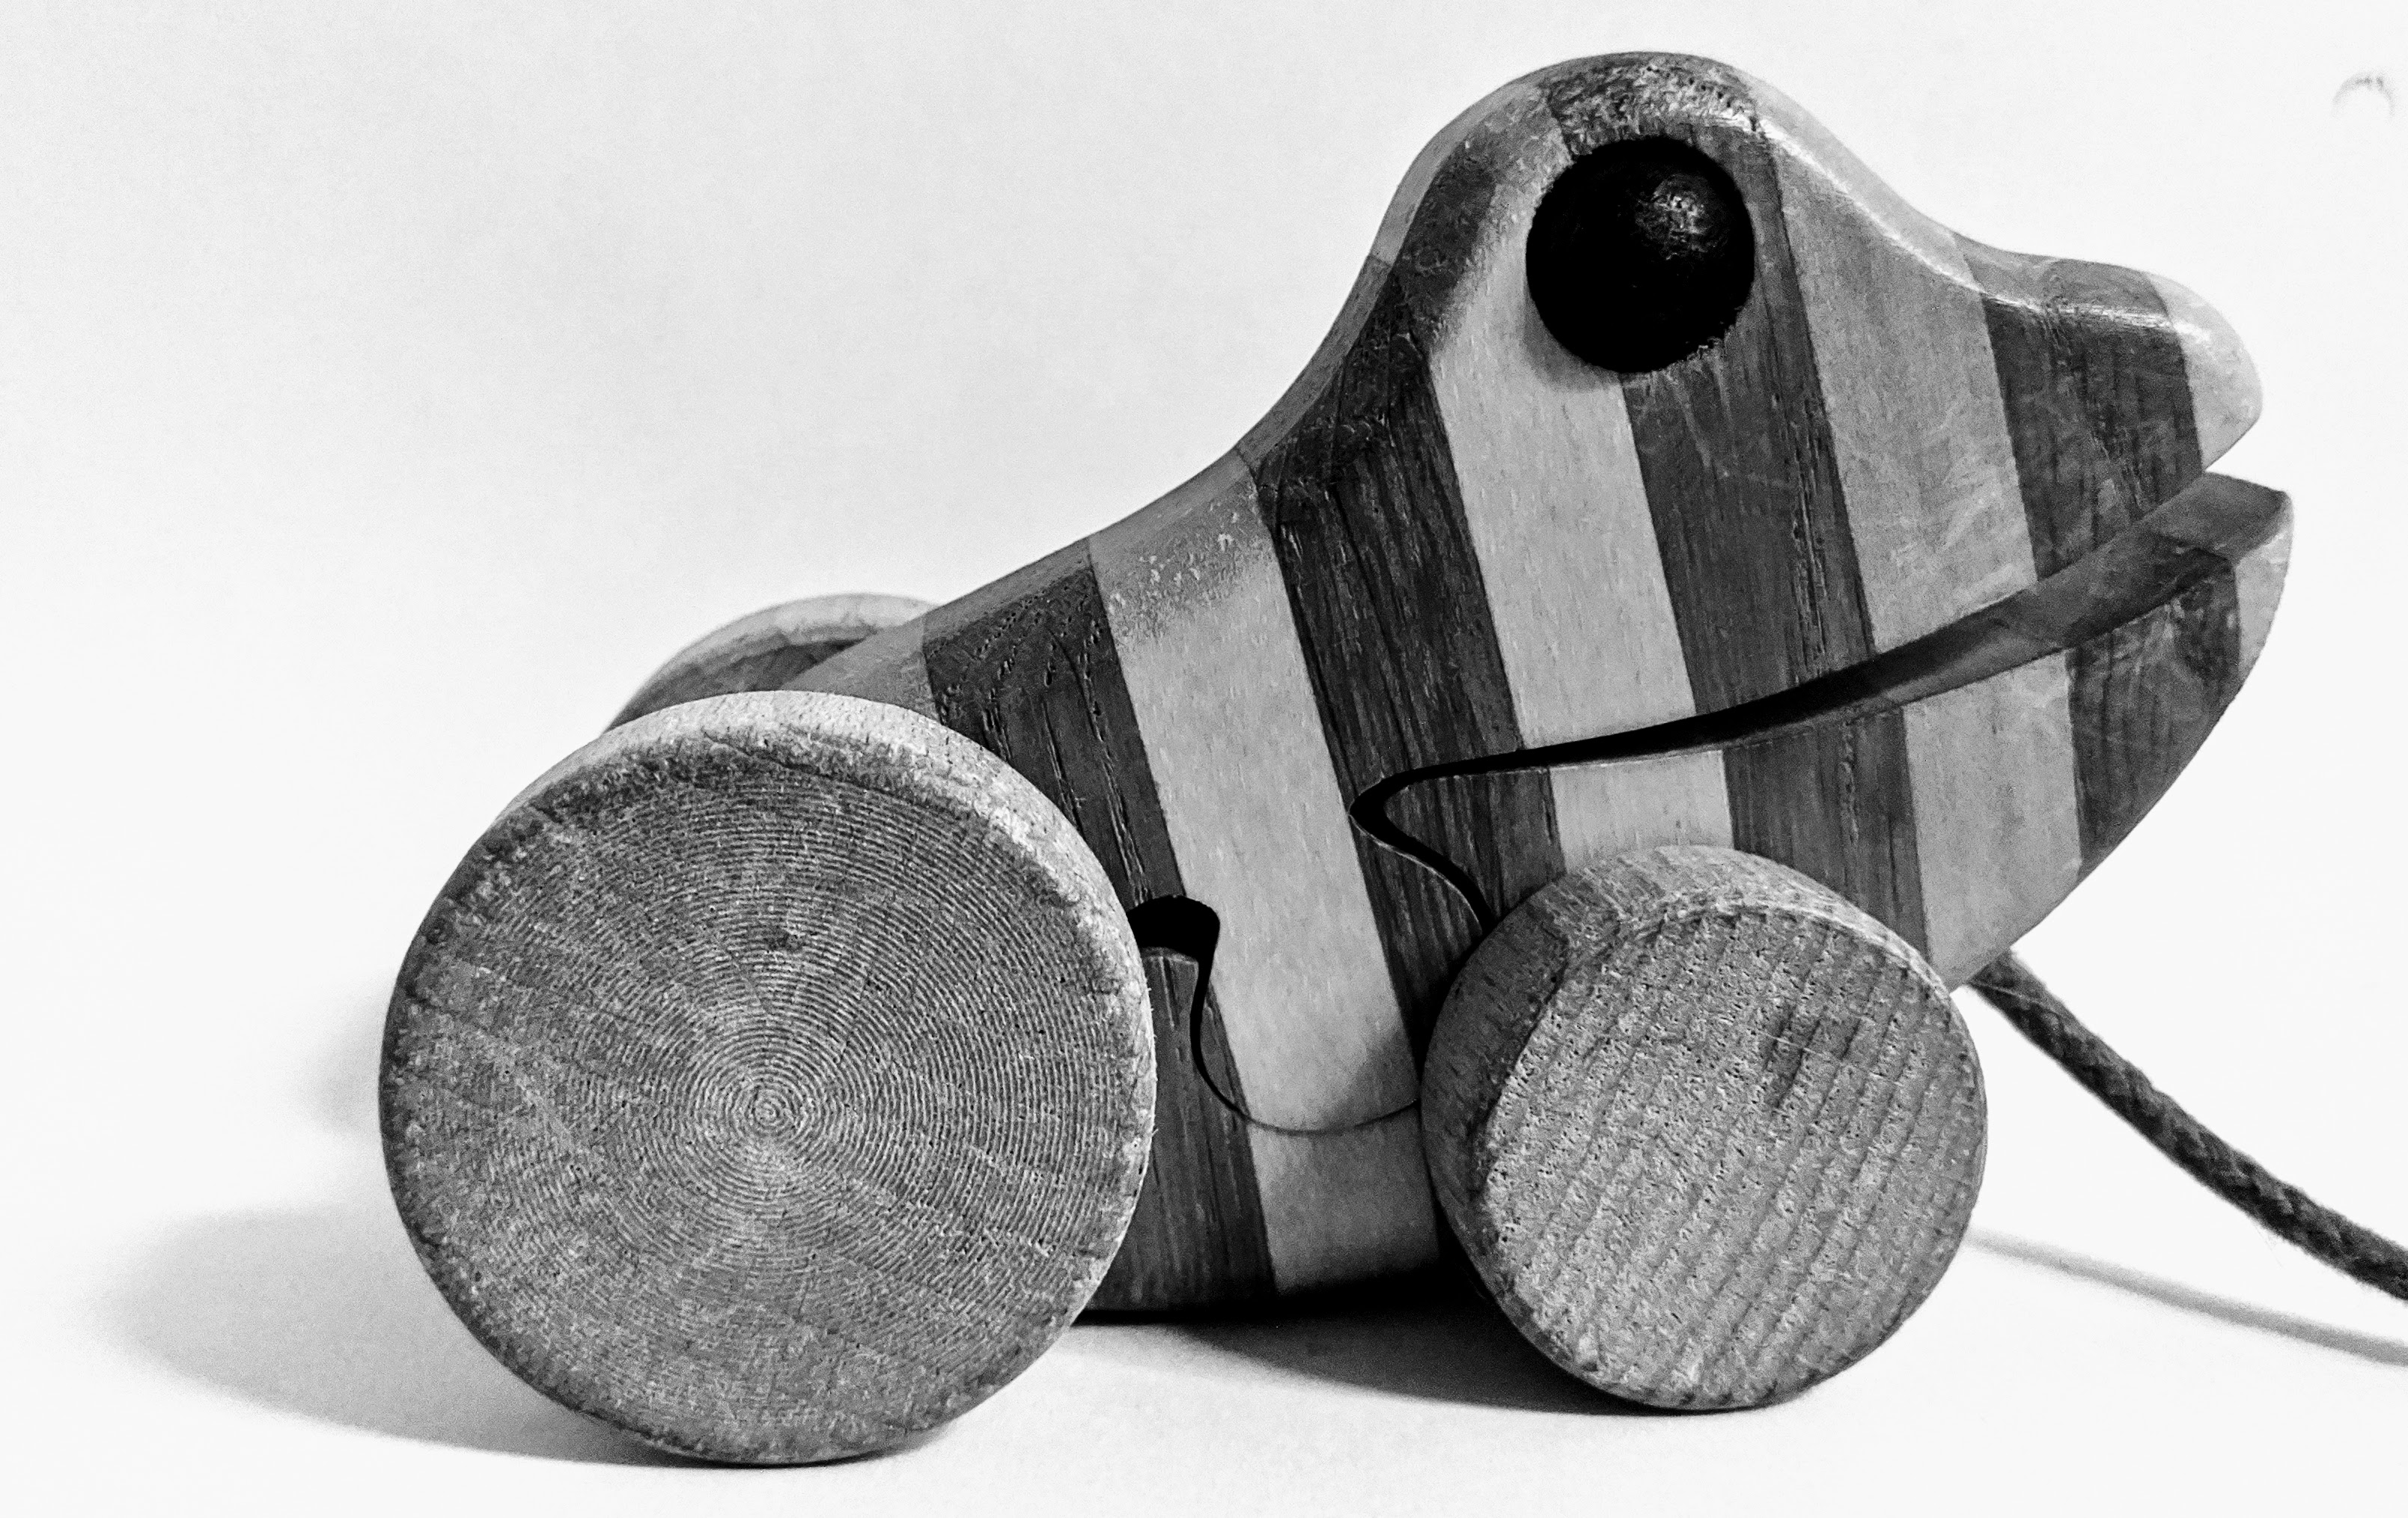
\includegraphics[height=3cm]{img/tigerente}
	\captionof*{figure}{example image recognition}
\end{center}

Supervised learning would fit a function that maps image pixels to recognizing the object in the image\\
from a set of possible objects (e.g. cat, dog, tiger, duck, frog, bird).
    
\end{frame}

\subsubsection{Unsupervised learning}

\begin{frame}{\subsecname: \subsubsecname}

We are given data that is made up of observations\pause~\textbf{only}. No other information.

\mode<presentation>{
\begin{center}
	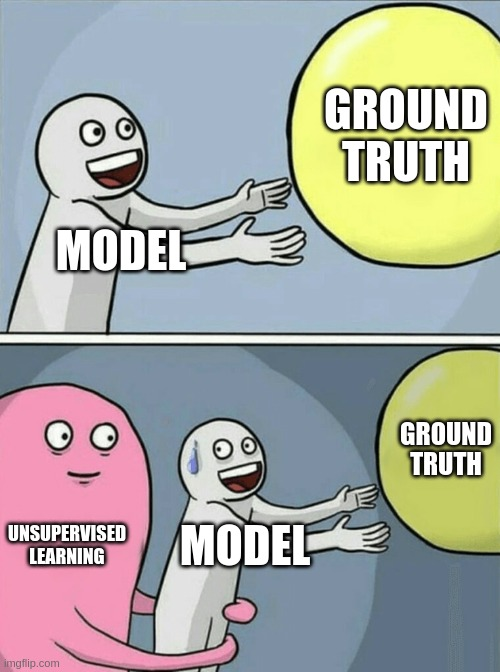
\includegraphics[width=4cm]{img/meme_nolabels}
\end{center}
}

\end{frame}

\begin{frame}{\subsubsecname}

\question{What can when we only have observations?}

\pause

\mode<article>
Unsupervised learning tries to 
\mode<all>
find interesting directions and/or structure in the data using only observations $\vec x \in \R^N$.

\begin{center}
	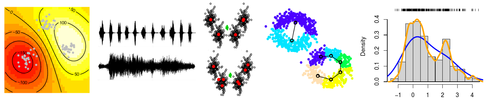
\includegraphics[width=9cm]{img/mi2}
\end{center}

``interesting'' and  ''structure'' is expressed through the objective model.

\end{frame}

\begin{frame}{\subsubsecname}

\underline{Data}:

A dataset of observations:
\begin{equation}
\label{eq:observations}
\vec X = 
\left(
\begin{array}{cccccc}
\Big| & \Big| & & \Big| & & \Big| \\[3mm]
\vec x^{(1)} & \vec x^{(2)} & \cdots & \vec x^{(\alpha)} & \cdots & \vec x^{(p)}\\[2mm]
\Big| & \Big| & & \Big| & & \Big|
\end{array}
\right) \in \R^{N \times p}
\end{equation}
\notesonly{
where $p$ denotes the number of observations (i.e. size of the dataset) and $N$ denotes the number of dimensions.}
\slidesonly{
where 
\begin{itemize}
\item[] $p$ \corresponds\, no. of observations (often \iid)
\item[] $N$ \corresponds\, no. of dimensions
\end{itemize}
}
\notesonly{
The samples are often assumed to be \iid, but algorithms for handling sequential data also exist.

Example: $\vec x$ could represent user ratings, pixel values in images.
}
\end{frame}
\begin{frame}

\underline{Objective model}:
\mode<presentation>{\vspace{5mm}}
\mode<article>{
An unsupervised learning algorithm is used to capture structure or directions in the data. This can be achieved by finding:
}
\begin{itemize}
\item the underlying distribution $P(\vec x)$ that generated this data (e.g. density estimation),
\item $\vec z := \vec f(\vec x)$, where $\vec z$ is a measure of 
\begin{itemize}
\item possible structure such as clustering or grouping in the data ($\vec z \in {0,\ldots,K-1}$), \\

and/or

\item possible directions in the data, by finding another continuous space for describing this data. \\

Example: dimensionality reduction, $\vec z \in \R^M$ with $M < N$.

\end{itemize}
\end{itemize}

\end{frame}
